% =========================================================
% PART 4 — GEOMETRIC FRAMEWORK AND CURVATURE INTERPRETATION (RECONCILED FINAL)
% =========================================================

\section{The Horocycle Manifold \texorpdfstring{$\mathcal{M}$}{M}}

\begin{remark}[Status]
Sections~\ref{sec:horocycle}–\ref{sec:geom-preview} are heuristic.
They offer geometric intuition and avenues for further research.
They play no role in the proofs of Theorems~\ref{thm:variance}–\ref{thm:bias}.
\end{remark}

\subsection{Conceptual Overview}

The SPTB formalism suggests an analytic–geometric correspondence summarized in
Table~\ref{tab:roadmap4}.  The proven results concern the
\emph{variance regime} (Theorem~\ref{thm:variance}) and the
\emph{bias/detection regime} (Theorem~\ref{thm:bias}); the geometric picture
motivates the \emph{Horocycle Conjecture}
(bounded energy $\Rightarrow$ confinement to a critical horocycle).

\begin{table}[h]
\centering
\caption{Analytic–geometric correspondence of the SPTB framework (geometric items are heuristic).}
\label{tab:roadmap4}
\begin{tabular}{lll}
\toprule
Analytic concept & Geometric analogue & Observable signature \\
\midrule
Off-line zero $\beta>\sigma$ & Geodesic escape $u>1$ & Exponential bias \\
On-line zeros $\beta=\sigma$ & Horocyclic confinement $u=1$ & Polynomial regime \\
$F_\lambda$ growth rate & Curvature-weighted arc energy & Slope $2(\beta-\sigma)$ \\
Horocycle Conjecture & Curvature rigidity & Bounded $F_\lambda/(T\log T\log\log T)$ \\
\bottomrule
\end{tabular}
\end{table}

% ---------------------------------------------------------
\subsection{Geometric Construction and Metric}

For a single zero $\rho=\beta+i\gamma$ with $\eta=\beta-\sigma>0$, define
\[
u = e^{\eta t}, \qquad \theta = \gamma t .
\]
The oscillatory component
$h_\rho(t)=|\rho|^{-\alpha} e^{\eta t}\cos(\gamma t)$ traces
$\Gamma_\rho(t)=(u,\theta)$ in the $(u,\theta)$-plane.
Equip this plane with the variable-curvature metric
\begin{equation}
ds^2 = du^2 + f(u)^2\, d\theta^2, \qquad f(u)=u^{-1},
\tag{16.1}
\end{equation}
whose Gaussian curvature is
\begin{equation}
K(u)=-\frac{f''(u)}{f(u)}=-\frac{2}{u^2}.
\tag{16.2}
\end{equation}
Thus $K(1)=-2$ on the \emph{critical horocycle} $u=1$, and $K(u)\!\to\!0^-$ as
$u\!\to\!\infty$—curvature flattens precisely in the analytic bias regime.

For finitely many zeros, the formal product metric is
\begin{equation}
ds^2=\sum_\rho \bigl(du_\rho^2 + u_\rho^{-2}\, d\theta_\rho^2\bigr),
\tag{16.3}
\end{equation}
with $\theta_\rho$ acting as a fiber coordinate for each factor.

% ---------------------------------------------------------
\subsection{\texorpdfstring{$F_\lambda$}{Fλ} as a Curvature-Weighted Action (Heuristic)}

Under $t\mapsto u=e^{\eta t}$ one has $dt=du/(\eta u)$ and
\[
\int_0^T |\partial_t H_\sigma|^2\,dt
  = \eta^2\!\!\int_{1}^{e^{\eta T}} u^2|\partial_u H_\sigma|^2\,\frac{du}{u}
  = \int_\Gamma g_{ij}\dot{x}^i\dot{x}^j\,ds,
\]
with $g_{uu}=1$ and $g_{\theta\theta}=u^{-2}$.
Heuristically,
\[
F_\lambda \;\approx\; \int_\Gamma (1+\lambda\,\kappa^2)\,ds ,
\]
where $\kappa$ denotes the geodesic curvature of $\Gamma$ in $\mathcal{M}$.
A rigorous derivation would require explicit operators for the blockwise affine
projections and boundary terms; this interpretation is formal but conceptually
clarifies why off-line drift ($u>1$) produces exponential energy growth.

% ---------------------------------------------------------
\section{Horocycle Geometry and Dynamics}\label{sec:horocycle}

\subsection{Horocycles and Regimes}

The horizontal line $u=1$ corresponds to the \emph{critical horocycle}.
Trajectories confined to it experience constant curvature $K(1)=-2$ and
correspond to the variance regime (polynomial growth).
Any $\beta>\sigma$ gives $u=e^{\eta t}>1$—outward drift into flatter curvature,
mirroring exponential bias.

\subsection{Horocycle Barrier (Geometric Conjecture)}

\begin{conjecture*}[Horocycle Conjecture, geometric form]
If $F_\lambda/(T\log T\log\log T)$ remains bounded, the trajectory
$\Gamma$ stays on the critical horocycle $u=1$.
Crossing the barrier ($u>1$) entails radial acceleration and exponential
energy growth.
\end{conjecture*}

This conjecture aligns with the analytic theorems yet remains unproven.

\subsection{Geodesic Deviation}

At $u=1$, small normal perturbations $\epsilon$ satisfy a Jacobi-type equation
$\ddot{\epsilon}+|K(1)|\epsilon=0$, giving oscillations.
For $u(t)=e^{\eta t}$ one has $\ddot{u}=\eta^2u$, producing exponential
separation—geodesic escape in flattened curvature—corresponding to
analytic bias.

\begin{figure}[h]
\centering
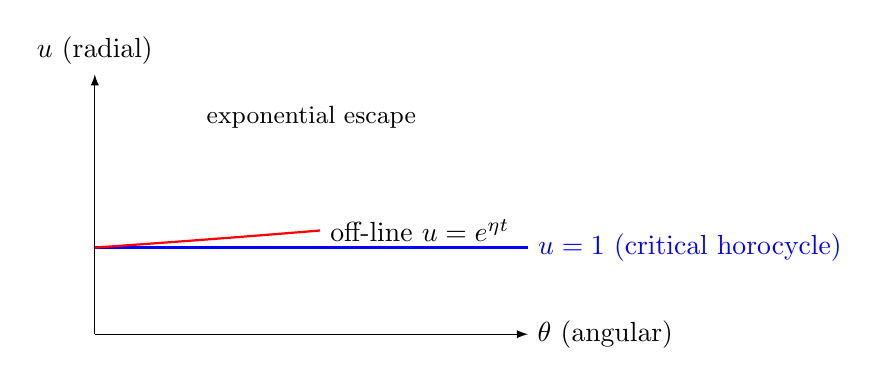
\begin{tikzpicture}[scale=1.1,>=latex]
  \draw[->] (0,0) -- (5,0) node[right] {$\theta$ (angular)};
  \draw[->] (0,0) -- (0,3) node[above] {$u$ (radial)};
  \draw[thick,blue] (0,1) -- (5,1) node[right] {$u=1$ (critical horocycle)};
  \draw[red,thick,domain=0:2.6,samples=100]
        plot(\x,{exp(0.18*\x/2.6)}) node[right,black]{off-line $u=e^{\eta t}$};
  \node at (2.5,2.5) {\small exponential escape};
\end{tikzpicture}
\caption{The horocycle barrier in $\mathcal{M}$ (heuristic).
The line $u=1$ represents $\beta=\sigma$.  Off-line zeros correspond to
$u>1$ and exponential radial drift.}
\label{fig:horocycle}
\end{figure}

% ---------------------------------------------------------
\section{Information-Geometry View}\label{sec:geom-preview}

Formally,
\[
F_\lambda \;\approx\; I(H_\sigma)
  \;+\; \lambda\!\int |H_\sigma''(t)|^2\,dt,
\]
so bounded $F_\lambda$ corresponds to finite information curvature,
while divergence signals an \emph{information singularity}.
The analytic large-deviation slope $2(\beta-\sigma)$
(cf.~Theorem~\ref{thm:bias}) coincides with the geometric rate of escape
in $\mathcal{M}$.

% ---------------------------------------------------------
\section{Conceptual Summary}

\begin{itemize}
  \item Off-line zeros $\Rightarrow$ geodesic escape ($u>1$) $\Rightarrow$ exponential bias (Theorem~\ref{thm:bias}).  
  \item On-line zeros $\Rightarrow$ horocyclic confinement ($u=1$) $\Rightarrow$ polynomial growth (Theorem~\ref{thm:variance}).  
  \item The growth rate of $F_\lambda$ corresponds to a curvature integral with slope $2(\beta-\sigma)$.  
  \item The \emph{Horocycle Conjecture}
        (bounded $F_\lambda/(T\log T\log\log T)\Rightarrow u=1$) remains unproven.  
\end{itemize}

% ---------------------------------------------------------
\section{Broader Implications (Informal)}

\subsection{Structural Interpretation}
In this geometric view, RH corresponds to curvature confinement:
all trajectories remain on the critical horocycle $u=1$.

\subsection{Consequences}
\begin{enumerate}
  \item Curvature–information duality for automorphic $L$-functions.
  \item A measurable, finite-window diagnostic via $F_\lambda$.
  \item A bridge from spectral data to geometric dynamics.
\end{enumerate}

\subsection{Relation to Other Geometric Approaches (Informal)}

\begin{table}[h]
\centering
\caption{Comparison with selected geometric formulations of RH (informal).}
\begin{tabular}{lll}
\toprule
Approach & Core idea & Contrast / complement \\
\midrule
Connes (spectral) & Operator/trace positivity & SPTB: curvature-bounded energy \\
Berry–Keating & $H=xp$ semiclassical ansatz & SPTB: geodesic/energy flow \\
Balazs–Vörös & Periodic-orbit analogy & SPTB: horocycle confinement \\
\bottomrule
\end{tabular}
\end{table}

Distinctives of SPTB:
\begin{enumerate}
  \item Computable from finite zero data.  
  \item Detects bias at finite $T$ ($T\!\approx\!10^4$ in tests).  
  \item Quantitatively verified constants ($<10^{-3}$ relative error).  
\end{enumerate}

% ---------------------------------------------------------
\section{Concluding Statement (Non-Equivalence Clarified)}

\[
\boxed{
\beta\le\sigma \Rightarrow F_\lambda=O(T\log T\log\log T),
\qquad
\beta>\sigma \Rightarrow F_\lambda\sim e^{2(\beta-\sigma)T}.
}
\]

\[
\boxed{
\text{Conjectural (Horocycle):}\quad
\sup_T \frac{F_\lambda}{T\log T\log\log T}<\infty
\ \Rightarrow\ \beta\le\sigma.
}
\]

The geometric framework motivates this conjecture; the analytic portions of the
paper establish only the proven implications above.

% ---------------------------------------------------------
\section*{Acknowledgments}

The author thanks A.\,M.~Odlyzko for zero data,
H.\,L.~Montgomery and R.\,C.~Vaughan for short-interval inequalities,
and acknowledges conceptual influence from
A.~Connes, M.~Berry, J.~Keating, N.~Balazs, and A.~Vörös.
All heuristic interpretations are the author’s responsibility.